\documentclass[a4paper,12pt,fleqn]{article}%fleqn pour aligner les equations à gauche
\usepackage{../../Styles/Cours}


\newcommand{\chnum}{Chapitre 3}
\newcommand{\chtitle}{Oxydoréduction}
\newcommand{\dtype}{Cours}

\begin{document}
\maketitle
\section*{Modéliser une transforation par une réaction d'oxydoréduction}

\begin{cours}
    \textbf{Un oxydant} est une espèce chimique capable de gagner un ou plusieurs électrons.\\
    \textbf{Un réducteur} est une espèce chimique capable de céder un ou plusieurs électrons.
\end{cours}
Une espèce chimique oxydants et une espèce chimique réductrice forment un \textbf{couple oxydant/réducteur} si l'on peut passer de l'une à l'autre par gain ou perte d'électrons. Les deux espèces sont dites conjuguées.
\begin{figure}[h!]
    \centering
    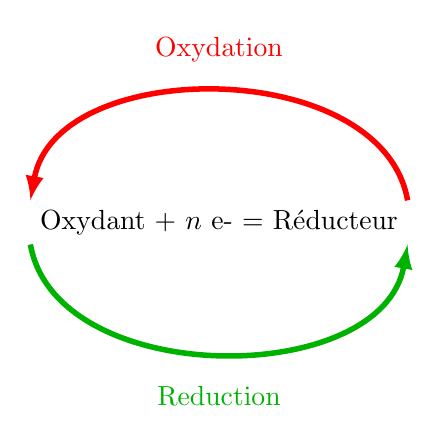
\begin{tikzpicture}
        \node (Eq) at (0,0){Oxydant + $n$ \ce{e-} = Réducteur};
        \draw[-latex,line width=.7mm,red] (Eq.north east) to[bend right = 80] (Eq.north west);
        \draw[-latex,line width=.7mm,green!70!black] (Eq.south west) to[bend right = 80] (Eq.south east);
        \node[red] (Ox) at (0,2.2){Oxydation};
        \node[green!70!black] (Red) at (0,-2.2){Reduction};
    \end{tikzpicture}
\end{figure}
\begin{cours}
    \textbf{Une oxydation correspond à une perte d'électrons.}\\
    \textbf{Une réduction correspond à un gain d'électrons.}
\end{cours}
Pour modéliser un échange de $n$ électrons entre l'oxydant et le réducteur d'un même couple, une demi-équation d'oxydoréduction peut être écrite :
$$\ce{Ox + n\cdot e^{-} = Red}$$
Lors d'une \textbf{réaction d'oxydorréduction}, il y a un transfert d'électrons du réducteur d'un couple à l'oxydant d'un second couple.\\
L'\textbf{équation d'une réaction d'oxydoréduction} est établie en combinant des demi-équations des deux couples mis en jeu de façon à ce que les élections n'interviennent pas.

\begin{exemple}
    \begin{itemize}
        \item \textbf{Établir la demi équation du couple \ce{Al^3+}/\ce{Al}}
        \item \textbf{Établir la demi équation du couple \ce{S2O8^2-}/\ce{SO4^2-}}
        \item \textbf{Établir la demi équation du couple \ce{MnO4^2-}/\ce{Mn^2+}}
    \end{itemize}
\end{exemple}
\end{document}